%        File: pres.tex
%     Created: Tues June 19 07:00 AM 2012 C
%
%\documentclass[11pt,handout]{beamer}
\documentclass[9pt]{beamer}

%\usepackage{bbding}
\usepackage{amsfonts}
\usepackage{graphicx}
\usepackage{subfigure}
\usepackage{booktabs} % nice rules for tables
\usepackage{microtype} % if using PDF
\usepackage{bigints}
\newcommand{\units}[1] {\:\text{#1}}%
\newcommand{\SN}{S$_N$}%{S$_\text{N}$}%{$S_N$}%
\DeclareMathOperator{\erf}{erf}


\usetheme[white]{Wisconsin}
%\title[short title]{long title}
\title[Cyclus and Cyder]{ Cyclus and Cyder : Open Source Tools for Fuel Cycle and Repository Analysis}
%\subtitle[short subtitle]{long subtitle}
\subtitle[Rising Stars]{MIT Rising Stars in Nuclear Science and Engineering 
Symposium} 
%\author[short name]{long name}
\author[Kathryn Huff]{Kathryn D.~Huff$^{1,2}$ \& UW-CNERG$^1$}
%\date[short date]{long date}
\date[03.05.2013]{March 5, 2013}
%\institution[short name]{long name}
\institute[UW-Madison]{$^1$University of Wisconsin-Madison \& $^2$Argonne National Laboratory}
%page numbers
\setbeamertemplate{footline}[page number]
%Those icons in the references are terrible looking
\setbeamertemplate{bibliography item}[text]
%I need some complimentary error funcitons... 
\DeclareMathOperator{\erfc}{erfc}


\begin{document}
%%%%%%%%%%%%%%%%%%%%%%%%%%%%%%%%%%%%%%%%%%%%%%%%%%%%%%%%%%%%%
%% From uw-beamer Here's a handy bit of code to place at 
%% the beginning of your presentation (after \begin{document}):
\newcommand*{\alphabet}{ABCDEFGHIJKLMNOPQRSTUVWXYZabcdefghijklmnopqrstuvwxyz}
\newlength{\highlightheight}
\newlength{\highlightdepth}
\newlength{\highlightmargin}
\setlength{\highlightmargin}{2pt}
\settoheight{\highlightheight}{\alphabet}
\settodepth{\highlightdepth}{\alphabet}
\addtolength{\highlightheight}{\highlightmargin}
\addtolength{\highlightdepth}{\highlightmargin}
\addtolength{\highlightheight}{\highlightdepth}
\newcommand*{\Highlight}{\rlap{\textcolor{HighlightBackground}{\rule[-\highlightdepth]{\linewidth}{\highlightheight}}}}
%%%%%%%%%%%%%%%%%%%%%%%%%%%%%%%%%%%%%%%%%%%%%%%%%%%%%%%%%%%%%
%%--------------------------------%%
\frame{
\titlepage
}
%%--------------------------------%%
\AtBeginSection[]{
\begin{frame}[c!]
  \frametitle{Outline}
  \tableofcontents[currentsection]
\end{frame}
}

%%--------------------------------%%
%%--------------------------------%%

\section{Cyder}
%Repository Capabilities within Systems Analysis Tools
%Conceptual Discussion of Disposal Environments

\begin{frame}[ctb!]
  \frametitle{Demonstration Case : Code Development}
  \footnotesize{
  The demonstration case is an empty software architecture in which to implement 
  the physical models. This demonstration has built and tested
  \begin{itemize}
    \item component module loading of models and data
    \item information passing between modules
    \item and database writing.
  \end{itemize}
  }
  \begin{figure}[htbp!]
    \begin{center}
      \includegraphics[height=.5\textheight]{cyder/images/componentLoading.eps}
    \end{center}
  \end{figure}
\end{frame}

\begin{frame}[ctb!]
  \frametitle{System Level Abstraction}
  \begin{figure}[h!]
      \includegraphics[width=\textwidth]{cyder/images/abstractionSystem.eps}
    \caption{System level abstraction seeks to determine the systems level 
    response to the change in models of subcomponents.}
  \end{figure}
\end{frame}

\begin{frame}
  \frametitle{Nested Components}
  Each component represents a 
  \begin{itemize}
    \item Waste Form
    \item Waste Package
    \item Buffer
    \item or Far Field (geologic medium).
  \end{itemize}
\end{frame}


\begin{frame}
  \frametitle{Nested Components}
  Each Component has : 
  \begin{itemize}
    \item a Geometry to describe its dimensions and location
    \item a NuclideModel for contaminant transport 
    \item a ThermalModel for heat transport
    \item a Parent Component at its external barrier
    \item one or more Daughter Components at its internal barrier
  \end{itemize}

  Components have other data members such as a Type (WF, WP, BUFFER, FF), a 
  material data table, a start date, etc. 
\end{frame}

\begin{frame}
  The NuclideModel in a Component can be interchangeably represented by any of 
  the four nuclide transport models. 
    \begin{itemize}
      \item Degradation Rate Based Failure Model
      \item Mixed Cell with Degradation, Sorption, Solubility Limitation
      \item Lumped Parameter Model
      \item 1D Advection Dispersion Solution
    \end{itemize}
\end{frame}

\subsection{Hydrogeologic Radionuclide Transport}
\begin{frame}
  \frametitle{Hydrologic Contaminant Transport}
  \footnotesize{
  In a saturated, reducing environment, contaminants are transported by 
  \textbf{dispersion} and \textbf{advection},  
    \begin{align}
      J &= J_{dis} + J_{adv}\nonumber\\
      &= -n(D_{mdis} + \tau D_m)\nabla C + nvC\nonumber\\ 
      &= -nD\nabla C + nvC \nonumber\\ 
      \intertext{which is, for uniform flow}
      &=\left(-nD_{xx} \frac{\partial C}{\partial x}
             + nv_xC \right)\hat{\imath}
             + \left( -nD_{yy} \frac{\partial C}{\partial y}
            \right)\hat{\jmath}
            + \left( -nD_{zz} \frac{\partial C}{\partial z}
            \right)\hat{k},
      \intertext{where}
      J_{dif} &= \mbox{ Total Dispersive Mass Flux }[kg/m^2/s]\nonumber\\
      J_{adv} &= \mbox{ Advective Mass Flux }[kg/m^2/s]\nonumber\\
      \tau &= \mbox{ Toruosity }[-] \nonumber\\
      n &= \mbox{ Porosity }[\%] \nonumber\\
      D_m &= \mbox{ Molecular diffusion coefficient }[m^2/s]\nonumber\\
      D_{mdis} &= \mbox{ Coefficient of mechanical dispersivity}[m^2/s]\nonumber\\
      D &= \mbox{ Effective Dispersion Coefficient }[m^2/s]\nonumber\\
      C &= \mbox{ Concentration }[kg/m^3],\nonumber\\
    \end{align}
    }

\end{frame}

\begin{frame}
  \frametitle{Hydrologic Contaminant Transport}
  \footnotesize{
  In addition to engineered barriers, their movement is constrained by 
  the solubility limit, 
    \begin{align}
      m_i &\leq V_w C_{sol,i},
    \intertext{and sorption,}
      S &=\frac{V_w(C_0 -C)}{m_s}
    \intertext{where}
      m_i &= \mbox{ mass of isotope i in volume }V_w [kg]\nonumber\\ 
      V_w &= \mbox{ volume of the solution }[m^3]\nonumber\\
      C_{sol,i} &= \mbox{ solubility limit, the maximum concentration of i }[kg_m^3]\nonumber\\
      S &= \mbox{ mass sorbed on the surface }[kg/kg]\nonumber\\
      C_0 &= \mbox{ initial concentration in the solution }[kg_m^3]\nonumber\\
      C &= \mbox{ equilibrium concentration in the solution }[kg/m^3]\nonumber\\
      m_s &= \mbox{ sediment mass }[kg].\nonumber
    \end{align}
    The function $S(C)$ is called a sorption isotherm. 
    }
\end{frame}

\begin{frame}
  \frametitle{Component Interfaces}
  \footnotesize{
  For uniform flow, the governing equation is,

  \begin{align}
    D_x \frac{\partial^2 C}{\partial x^2} +
    D_y \frac{\partial^2 C}{\partial y^2} +
    D_z \frac{\partial^2 C}{\partial z^2} +
    v_x \frac{\partial C}{\partial x}  = R_f \frac{\partial C}{\partial t}.  
    \label{unidirflow}
  \end{align}

  \begin{figure}[htp!]
    \begin{center}
      \def\svgwidth{\textwidth}
      \input{cyder/images/flow.eps_tex}
    \end{center}
    \caption{The boundaries between components are robust interfaces defined by 
    Source Term, Dirichlet, Neumann, and Cauchy boundary conditions.}
    \label{fig:flow}
  \end{figure}
  }
\end{frame}

\begin{frame}
  \frametitle{Boundary Conditions}
  \footnotesize{
    \textbf{First, specified-head or Dirichlet type} boundary conditions define a specified species 
    concentration
    
    \begin{align}
      C(\vec{r},t) = C_0(\vec{r},t)\hspace{1mm}\mbox{ for } \left( \vec{r} \right) \in 
      \Gamma.
    \end{align}
    
    \textbf{Second, specified-flow, or Neumann type} boundary conditions describe a full set of 
    concentration gradients 
    
    \begin{align}
      \frac{\partial C(\vec{r},t)}{\partial r} &= nD\vec{J}(t) \hspace{1mm}\mbox{ for } 
      \vec{r} \in \Gamma.
      \intertext{where}
      \vec{r} &= \mbox{ position vector }\nonumber\\
      \Gamma &= \mbox{ domain boundary }\nonumber\\
      \vec{J}(t) &= \mbox{ solute mass flux } [kg/m^2\cdot s].\nonumber
    \end{align}
    
    \textbf{Third, head-dependent, or Cauchy type}, defines a solute 
    flux along the boundary,
    
    \begin{align}
      -D\frac{\partial C}{\partial x} + v_xC &= v_xC(\vec{r},t).
      \intertext{where}
      D &= \mbox{ hydrodynamic dispersion coefficient } [m^2/s]\nonumber\\
      v_x &= \mbox{ outward fluid flux} [m/s]\nonumber\\
    \end{align}  
  }
\end{frame}

\begin{frame}
  \frametitle{Radionuclide Transport: Mixed Cell}
  % Waste Form
  \begin{figure}[h!]
    \begin{center}
      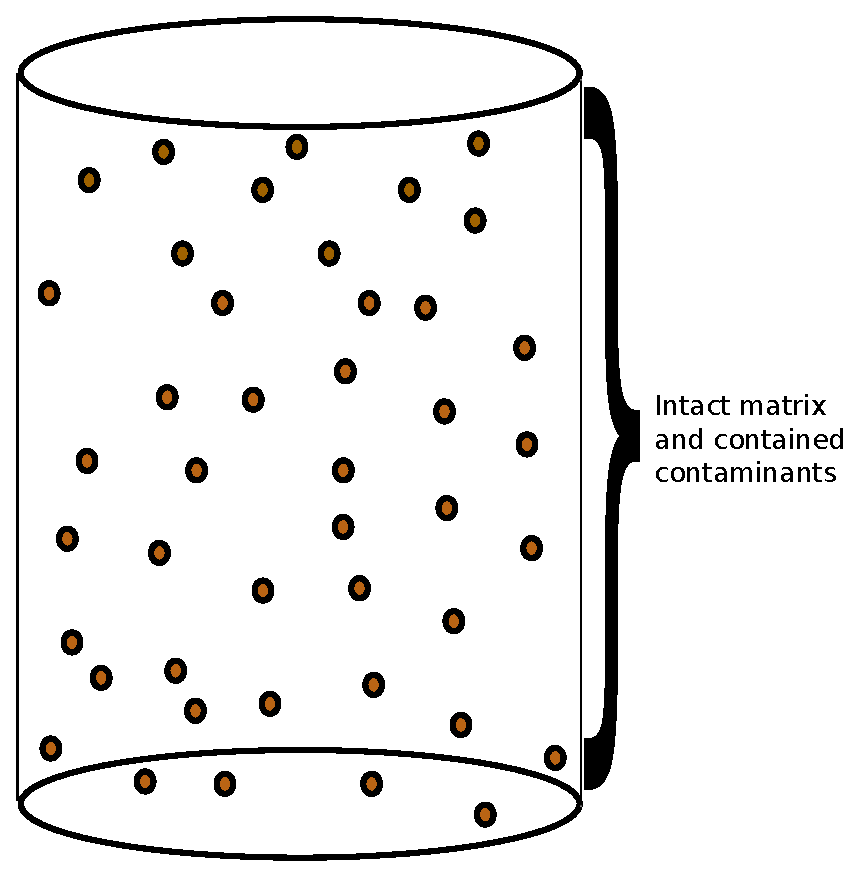
\includegraphics[height=.6\textwidth]{cyder/images/mixed_cell_whole.eps}
    \end{center}
  \end{figure}
\end{frame}

\begin{frame}[ctb!]
  \frametitle{Radionuclide Transport: Mixed Cell}
  % Waste Form
  \begin{figure}[h!]
    \begin{center}
      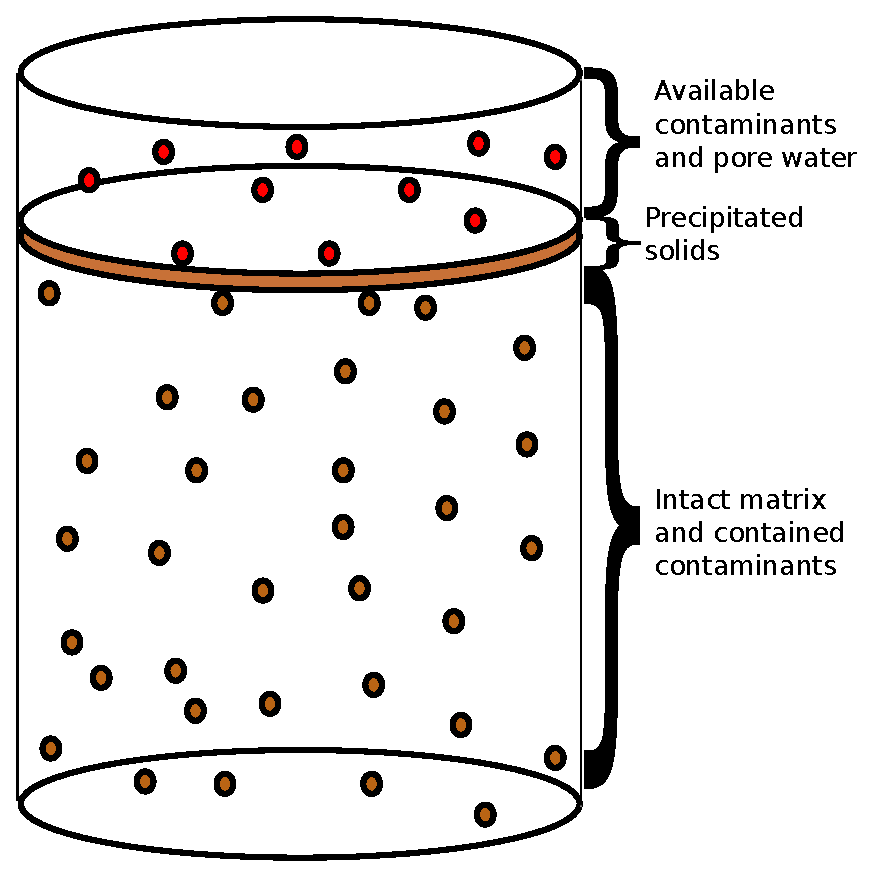
\includegraphics[height=.6\textwidth]{cyder/images/mixed_cell_degraded.eps}
    \end{center}
  \end{figure}
\end{frame}

\begin{frame}
  \frametitle{Radionuclide Transport: Rate Based Congruent Release}
  \footnotesize{
  Contaminants are released congruently with degradation of the component.

  That is, for a rate of $\epsilon [\%]$ per year, where the initial condition is some 
  contained mass, $m_0$, the boundary conditions supplied to external components 
  at the outer boundary $r_{bc}$are :

  \begin{align}
    \intertext{Source Term}
    \dot{m} &= \epsilon m_0
    \intertext{Dirichlet}
    C(r_{bc}) &= \dot{m}/V_w 
    \intertext{Neumann}
    \frac{\partial C}{\partial r} &= ( \dot{m}/V_w - C_{ext} )/(r_{ext} - r_{in})
    \intertext{Cauchy}
    -D \frac{\partial C}{\partial x}\big|_{x=x_{bc}} + v_xc &= vC(x_{bc}) 
  \end{align}
  }
\end{frame}

\begin{frame}
  \frametitle{Radionuclide Transport: Lumped Parameter Transport Model}

\begin{figure}[htbp!]
  \begin{center}
    \def\svgwidth{\textwidth}
    \input{cyder/images/lumpedseries.eps_tex}
  \end{center}
  \caption{ For systems in which the flow can be assumed constant, it is 
  possible to model a system of volumes as a connected lumped paramter models 
  according to a relationship between the incoming concentration, $C_{in}(t)$, 
  and the outgoing concentration, $C_{out}(t)$.}
  \label{fig:lumpedseries}
\end{figure}
\footnotesize{
  \begin{align}
  C_{out}(t) &= \int_0^\infty C_{in}(t-t')g(t')e^{-\lambda t'}dt'
  \label{lumped2}
  \intertext{where}
  t'  &= \mbox{ time of entry }[s]\nonumber\\
  t-t'  &= \mbox{ transit time }[s]\nonumber\\
  g(t-t')  &= \mbox{ response function, a.k.a. transit time 
  distribution}[-]\nonumber]\\
  \lambda &= \mbox{ radioactive decay constant, 1 to neglect}[s^{-1}]
\end{align}
}
\end{frame}


\begin{frame}
  \frametitle{Radionuclide Transport: Lumped Parameter Transport Model}
\footnotesize{
Selection of the response function is usually based on experimental tracer 
results. Canonical forms include :
\begin{align}
  \mbox{the Piston Flow Model (PFM), } g(t') &= \delta{(t'-t_t))}\\
  \mbox{ the Exponential Model (EM), } g(t') &= 
  \frac{1}{t_t}e^{-\frac{t'}{t_t}}\\
  \mbox{ and the Dispersion Model (DM), } g(t') &= \frac{\left[ \left( \frac{t\pi t'}{t_t Pe} \right) 
  (\frac{1}{t'})e^{- \left( 1- \frac{t'}{t_t}  \right)^2} 
  \right]}{\frac{4t'}{t_tPe}}, 
  \intertext{where}
  Pe  &= \mbox{ Peclet number }[-]\nonumber\\
  t_t  &= \mbox{ mean tracer age }[s]\nonumber\\
    &= t_w \mbox{ if there are no stagnant areas}\nonumber\\
  t_w  &= \mbox{ mean residence time of water}[s].\nonumber\\
\intertext{The solutions to these for constant concentration at the source 
boundary give}
  C(t) &=\begin{cases}
    PFM & C_0e^{-\lambda t_t}\\
    EM  & \frac{C_0}{1+\lambda t_t}\\
    DM  & \frac{C_0e^{Pe\sqrt{\left( 1-(1+\frac{4\lambda t_t}{Pe})\right)}}}{2}\\
  \end{cases}
  \label{lumpedsolns}
\end{align}
}
\end{frame}

\begin{frame}
  \frametitle{Radionuclide Transport: 1D Semi-Infinite, Cauchy B.C.}
  \footnotesize{
\begin{figure}[htbp!]
  \begin{center}
    \def\svgwidth{.5\textwidth}
    \input{cyder/images/1dinf.eps_tex}
  \end{center}
  \caption{A one dimensional, semi-infinite model, unidirectional flow,
  solution with Cauchy and Neumann B.C.s}
  \label{fig:1dinf}
\end{figure}
The solution is given (Leij and van Genuchten, \cite{leij_analytical_1991})  as :
\begin{align}
  C(x,t) = \frac{C_0}{2}\Bigg[&\erfc{\frac{L-v_xt}{2\sqrt{D_Lt}}} 
  + \frac{1}{2} \left(\frac{v_x^2t}{\pi D_L}\right)^{1/2}e^{\frac{-( L - 
  v_xt)^2}{4D_Lt}}\nonumber\\
  &- \frac{1}{2}\left( 
  1+\frac{v_xL}{D_L}+\frac{v_x^2t}{D_L}\right)e^\frac{v_xL}{D_L}\erfc{\left[\frac{L-V_xt}{2\sqrt{D_Lt}}\right]} 
  \Bigg]
  \end{align}
  }
\end{frame}


\begin{frame}[ctb]
\frametitle{Sensitivity Analysis with the Clay Generic Disposal System Model}

Recall : Abstraction process uses results from more detailed models to improve 
speed and accuracy of analytical models. In this case, sensitivity analyses were 
conducted using the Used Fuel Disposition Campaign's Clay Generic Disposal System 
Model \cite{huff_key_2012} in order to inform the analytic models just discussed.

\begin{table}[ht!]
\centering
\footnotesize{
\begin{tabular}{|l|l|l|r|r|}
\multicolumn{5}{c}{\textbf{Simulation Cases}}\\
\hline
\textbf{Case} & \textbf{Parameter} & \textbf{Units} & \textbf{Min. Value} & \textbf{Max. Value}\\
\hline
I     & $D_{eff}$    & $[m^2\cdot s^{-1}]$       & $10^{-8}$    &  $10^{-5}$ \\
      & Inventory              & [MTHM]         & $10^{-4}$    &  $10^1$ \\
\hline
II    & $V_{adv, y}$ & $[m \cdot yr^{-1}]$       & $6.31\times10^{-8}$  &  $6.31\times10^{-4}$ \\
      & $D_{eff}$    & $[m^2\cdot s^{-1}]$       & $10^{-8}$    &  $10^{-5}$ \\
\hline
III   & $S_i$        & $[mol\cdot m^{-3}]$       & $(1\times10^{-9})\langle S_i\rangle $    &  $(5\times10^{10})\langle S_i\rangle $ \\
\hline
IV    & $K_{d,i}$    & $[m^3\cdot kg^{-1}]$       & $(1\times10^{-9})\langle K_{d,i}\rangle $    &  $(5\times10^{10})\langle K_{d,i}\rangle $ \\
\hline
V     & $R_{WFDeg.}$           & $[yr^{-1}]$       & $10^{-9}$    &  $10^{-2}$ \\
      & Inventory              & [MTHM]         & $10^{-4}$    &  $10^1$ \\
\hline 
VI    & $t_{WPFail}$        & $[yr]$         & $10^3$    &  $10^7$ \\
      & $D_{eff}$           & $[m^2\cdot s^{-1}]$       & $10^{-8}$    &  $10^{-5}$ \\
\hline
\end{tabular}
\caption{Each dual and single parameter simulation case had 40 simulation 
groups of 100 realizations each.}
\label{tab:Cases}
}
\end{table}



\end{frame}


\begin{frame}[ctb]
\frametitle{Solubility Sensitivity}
\begin{figure}[ht]
  \centering
  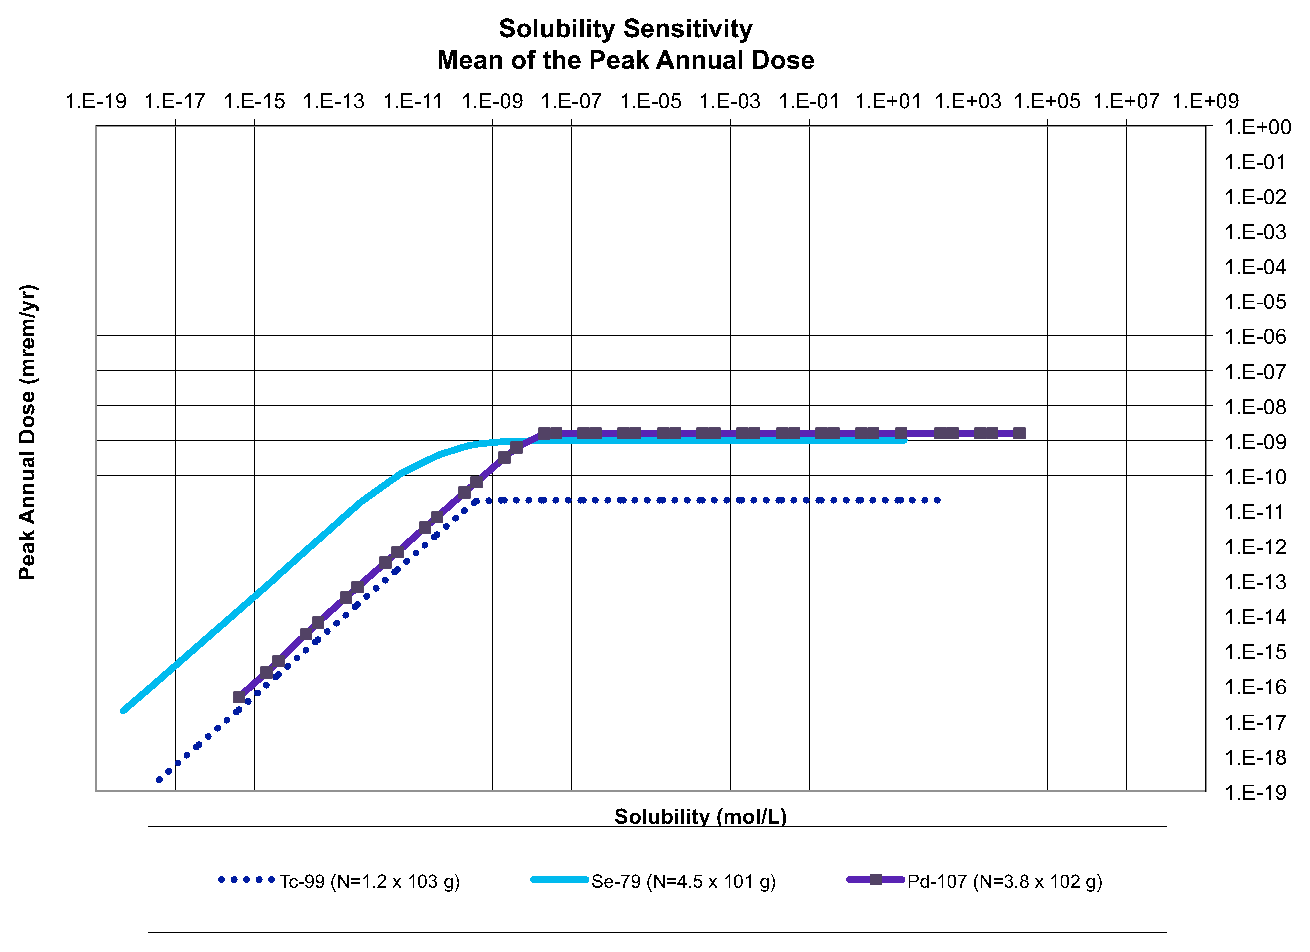
\includegraphics[height=60mm]{cyder/images/Solubility_Summary.eps}
  \caption{Generated with the Used Fuel Disposition Campaign's Generic Disposal 
  System Model for Clay, this graph demonstrates solubility limit sensitivity. 
  The peak annual dose due to an inventory, $N$, of each isotope.}
  \label{fig:SolSum}
\end{figure}
\end{frame}

\begin{frame}[ctb]
\frametitle{Retardation Sensitivity}
\begin{figure}[ht]
  \centering
  \includegraphics[height=60mm]{cyder/images/Partitioning_Summary.eps}
  \caption{Generated with the Used Fuel Disposition Campaign's Generic Disposal 
  System Model for Clay, this graph demonstrates $K_d$ sensitivity. 
  The peak annual dose due to an inventory, $N$, of each isotope.}
  \label{fig:KdSum}
\end{figure}
\end{frame}



\begin{frame}[ctb!]
  \frametitle{Summary}
  Completed infrastructure includes :
  \begin{itemize}
  \item[$\checkmark$] Generic Repository infrastructure 
  \item[$\checkmark$] Component loading
  \item[$\checkmark$] Component Geometry and placement
  \item[$\checkmark$] Output tables
  \item[$\checkmark$] Rudimentary plotting scripts
  \item[$\checkmark$] Fundamental base cases demonstrate nuclide transport 
  \item[$\checkmark$] Lots of tests
  \end{itemize}
  Further NuclideModel implementation, testing, and sensitivity analyses 
  include:
  \begin{itemize}
  \item[$\square$] Record Far Field contaminant data in the database 
  \item[$\square$] Robustly check for mass conservation with FF included 
  \item[$\square$] Record Component parent IDs in the database
  \item[$\square$] Clean up plotting script 
  \item[$\square$] Run longer term sensitivity analyses on sorption and solubility 
  \item[$\square$] Run base cases for Lumped Parameter model
  \item[$\square$] Run base cases for 1D Analytic model
  \item[$\square$] Compare results robustly with GoldSim models
  \item[$\square$] More tests
  \end{itemize}

\end{frame}





\begin{frame}[ctb!]
  \frametitle{Acknowledgements}  
\begin{figure}[htp!]
\begin{center}
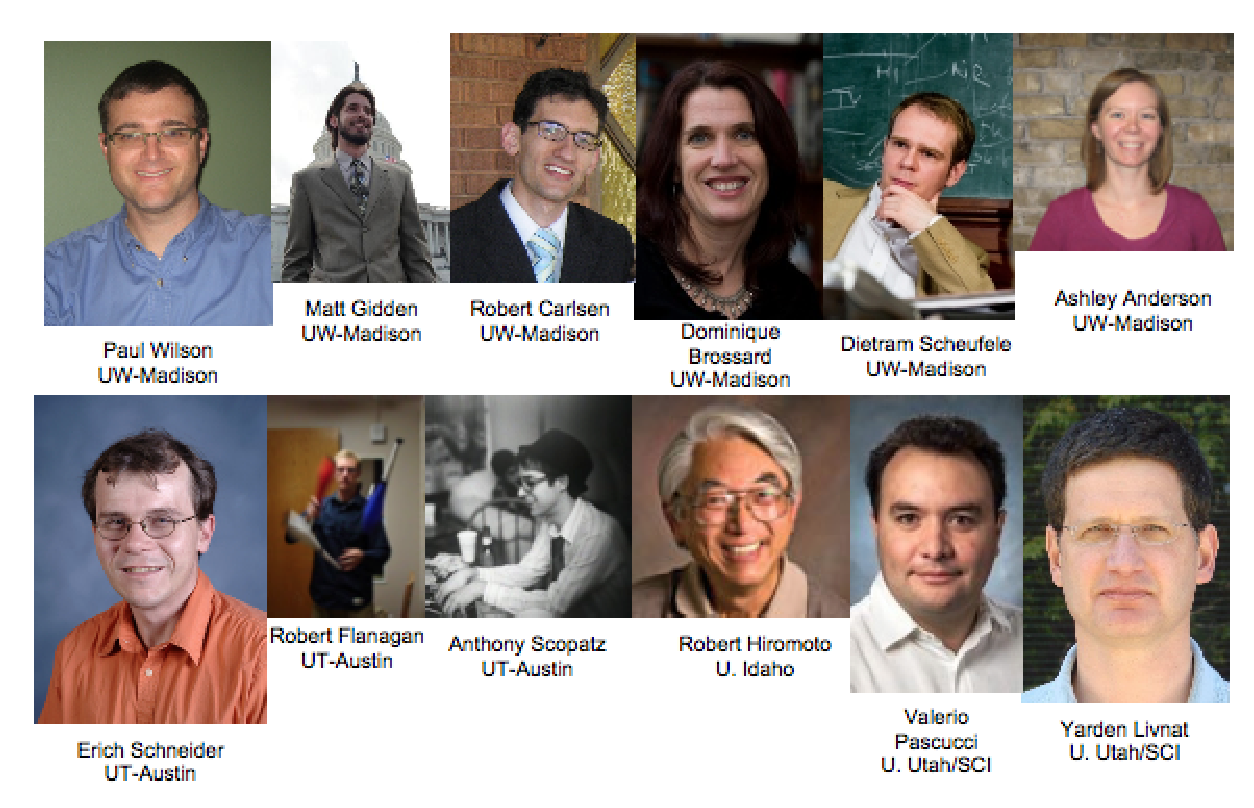
\includegraphics[width=0.6\textwidth]{images/ngfcspics.eps}
\end{center}
\caption{The rest of the Next Generation Fuel Cycle Simulator Team.}
\label{fig:ngfcspics}
\end{figure}

\end{frame}

\begin{frame}[ctb!]
  \frametitle{Acknowledgements}  
  My work at Argonne is supported by the Office of Science Laboratory graduate 
  program, the Used Fuel Disposition Campaign, and my supervisor Mark Nutt.

  This work is supported by the following institutions. 

  \begin{figure}[htp]
    \centering
    \subfigure{\label{figur:1}
\includegraphics[height=20mm]{UW_crest.ps}}
    \subfigure{\label{figur:2}
\includegraphics[height=20mm]{neup_logo_large.eps}}
    \subfigure{\label{figur:3}
\includegraphics[height=20mm]{nsf_logo.eps}}
    \\ 
    \subfigure{\label{figur:4}
\includegraphics[height=20mm]{AnlLogo.eps}}
    \subfigure{\label{figur:5}
\includegraphics[height=20mm]{USNRC.eps}}
    \\
  \end{figure}

\end{frame}

%%--------------------------------%%
%%--------------------------------%%
\begin{frame}[allowframebreaks]
  \frametitle{References}
  \bibliographystyle{plain}
  {\footnotesize \bibliography{pres} }

\end{frame}

%%--------------------------------%%





\end{document}




